%%%%%%%%%%%%%%%%%%%%%%%%%%%%%%%%%%%%%%%%
% Wenneker Assignment
% LaTeX Template
% Version 2.0 (12/1/2019)
%
% This template originates from:
% http://www.LaTeXTemplates.com
%
% Authors:
% Vel (vel@LaTeXTemplates.com)
% Frits Wenneker
%
% License:
% CC BY-NC-SA 3.0 (http://creativecommons.org/licenses/by-nc-sa/3.0/)
% 
%%%%%%%%%%%%%%%%%%%%%%%%%%%%%%%%%%%%%%%%%

%----------------------------------------------------------------------------------------
%	PACKAGES AND OTHER DOCUMENT CONFIGURATIONS
%----------------------------------------------------------------------------------------

\documentclass[11pt]{scrartcl} % Font size

%%%%%%%%%%%%%%%%%%%%%%%%%%%%%%%%%%%%%%%
% Wenneker Assignment
% Structure Specification File
% Version 2.0 (12/1/2019)
%
% This template originates from:
% http://www.LaTeXTemplates.com
%
% Authors:
% Vel (vel@LaTeXTemplates.com)
% Frits Wenneker
%
% License:
% CC BY-NC-SA 3.0 (http://creativecommons.org/licenses/by-nc-sa/3.0/)
% 
%%%%%%%%%%%%%%%%%%%%%%%%%%%%%%%%%%%%%%%%%

%----------------------------------------------------------------------------------------
%	PACKAGES AND OTHER DOCUMENT CONFIGURATIONS
%----------------------------------------------------------------------------------------
\usepackage{xcolor}   % for \textcolor
\usepackage{comment}

\usepackage{amsmath, amsfonts, amsthm} % Math packages

\usepackage{listings} % Code listings, with syntax highlighting
\usepackage{verbatim} % Directly from txt file

\usepackage[english]{babel} % English language hyphenation
\usepackage{tikz} 
\usepackage{neuralnetwork} 
\usepackage{graphicx} % Required for inserting images
\graphicspath{{Figures/}{./}} % Specifies where to look for included images (trailing slash required)
\usepackage{setspace}  % allows linespacing changes
\usepackage{tabularx} % for tables

\usepackage{booktabs} % Required for better horizontal rules in tables

\numberwithin{equation}{section} % Number equations within sections (i.e. 1.1, 1.2, 2.1, 2.2 instead of 1, 2, 3, 4)
\numberwithin{figure}{section} % Number figures within sections (i.e. 1.1, 1.2, 2.1, 2.2 instead of 1, 2, 3, 4)
\numberwithin{table}{section} % Number tables within sections (i.e. 1.1, 1.2, 2.1, 2.2 instead of 1, 2, 3, 4)

\setlength\parindent{0pt} % Removes all indentation from paragraphs

\usepackage{enumitem} % Required for list customisation
\setlist{noitemsep} % No spacing between list items

%----------------------------------------------------------------------------------------
%	DOCUMENT MARGINS
%----------------------------------------------------------------------------------------

\usepackage{geometry} % Required for adjusting page dimensions and margins

\geometry{
	paper=a4paper, % Paper size, change to letterpaper for US letter size
	top=2.5cm, % Top margin
	bottom=3cm, % Bottom margin
	left=3cm, % Left margin
	right=3cm, % Right margin
	headheight=0.75cm, % Header height
	footskip=1.5cm, % Space from the bottom margin to the baseline of the footer
	headsep=0.75cm, % Space from the top margin to the baseline of the header
	%showframe, % Uncomment to show how the type block is set on the page
}

%----------------------------------------------------------------------------------------
%	FONTS
%----------------------------------------------------------------------------------------

\usepackage[utf8]{inputenc} % Required for inputting international characters
\usepackage[T1]{fontenc} % Use 8-bit encoding

\usepackage{fourier} % Use the Adobe Utopia font for the document

%----------------------------------------------------------------------------------------
%	SECTION TITLES
%----------------------------------------------------------------------------------------

\usepackage{sectsty} % Allows customising section commands

\sectionfont{\vspace{6pt}\centering\normalfont\scshape} % \section{} styling
\subsectionfont{\normalfont\bfseries} % \subsection{} styling
\subsubsectionfont{\normalfont\itshape} % \subsubsection{} styling
\paragraphfont{\normalfont\scshape} % \paragraph{} styling

%----------------------------------------------------------------------------------------
%	HEADERS AND FOOTERS
%----------------------------------------------------------------------------------------

\usepackage{scrlayer-scrpage} % Required for customising headers and footers

\ohead*{} % Right header
\ihead*{} % Left header
\chead*{} % Centre header

\ofoot*{} % Right footer
\ifoot*{} % Left footer
\cfoot*{\pagemark} % Centre footer
 % Include the file specifying the document structure and custom commands
\usepackage{cite}

\usepackage{hyperref}

%----------------------------------------------------------------------------------------
%	TITLE SECTION
%----------------------------------------------------------------------------------------

\title{	
	\normalfont\normalsize
	\textsc{Intelligent Robotics, Portland State University}\\ % Your university, school and/or department name(s)
	\vspace{25pt} % Whitespace
	\rule{\linewidth}{0.5pt}\\ % Thin top horizontal rule
	\vspace{20pt} % Whitespace
	{\huge Winter Report}\\ % The assignment title
	\vspace{4pt} % Whitespace
	{\large Quaternion Attitude Control of a Simulated Airplane}\\ % The assignment title
	\vspace{12pt} % Whitespace
	\rule{\linewidth}{2pt}\\ % Thick bottom horizontal rule
	\vspace{12pt} % Whitespace
}

\author{\LARGE Trenton Ruf} % Your name
\date{\normalsize \today} % Today's date (\today) or a custom date

\begin{document}
\maketitle % Print the title
%\renewcommand\thesubsection{\Alph{subsection}}
%\renewcommand\thesubsection{\Roman{subsection}}
%\doublespacing
%\singlespace
%\onehalfspacing
%\setstretch{1.25}

%\begin{doublespace}
%\end{doublespace}

%\vspace*{\fill}
%\clearpage
%\vspace*{\fill}


%\vspace*{\fill}
\renewcommand\thesubsection{\Roman{subsection}}
\section{Changes to last term's code}
I made the fuzzy-altitude controller from last term into a ROS service server. This is to control the attitude setpoint and enable/disable the controller from a separate ROS node. My plan is to have the altitude and attitude controller nodes given commands by a master "State Machine" node.


\section{Quaternion control}

\subsection{Why quaternion?}
Traditional attitude controllers for aircraft use Euler angles to determine orientation. Euler angles are great because they are intuitive to conceptualize and implement, but they have a major drawback. When an aircraft pitches up 90 degrees; yaw changes can no longer be tracked. Effectively losing a degree of freedom. Quaternions do not have this issue. But unlike Euler angles they are (in my experience) near impossible to visualize and conceptualize. Though surprisingly easy to implement as a controller.

\subsection{controller layout}

\begin{figure}[ht!] % [h] forces the figure to be output where it is defined in the code (it suppresses floating)
	\centering
	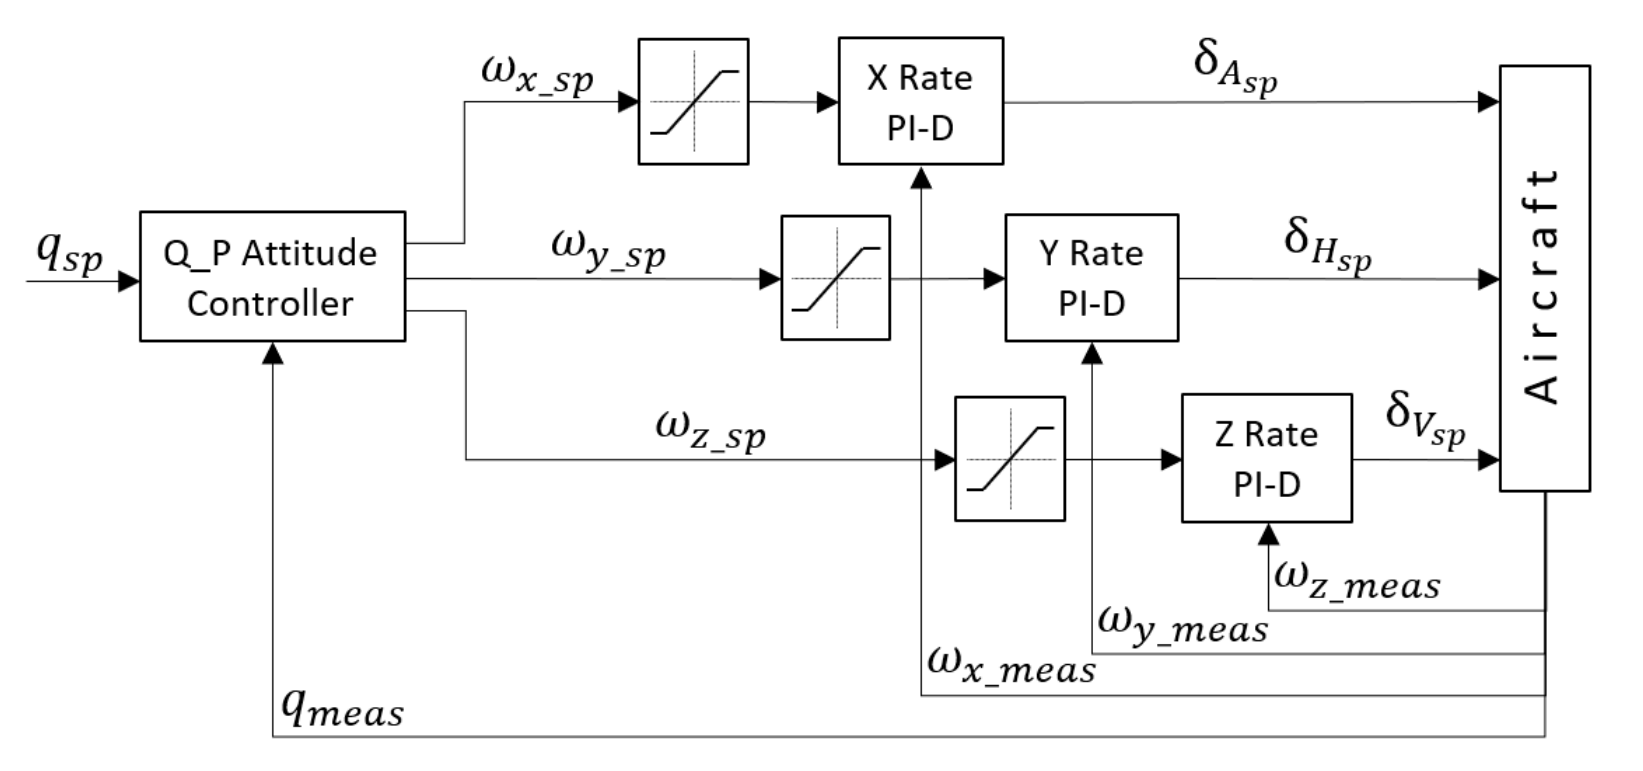
\includegraphics[width=0.9\columnwidth]{QuatSchematicPID.png} 
	\caption{Quaternion-Based controller schematic from ~\cite{quat}}
\end{figure}

The quaternion attitude controller was modeled after the one described in 

\underline{Quaternion Attitude Control System of Highly Maneuverable Aircraft} ~\cite{quat}. It is a cascading controller that takes a quaternion setpoint ($q_{sp}$) and quaternion measured ($q_{meas}$) as the initial inputs to a proportional controller. The outputs of the proportional controller are angular velocity setpoints for their respective x, y, and z access PID controllers. The secondary inputs to these PIDs are the current measured angular velocities. The final outputs are the positions of the airplane control surfaces (rudder, aileron, and elevator).

\subsection{step by step}
For the mathematical notation and in depth look for each step, please check pages 4-6 of \underline{Quaternion Attitude Control System of Highly Maneuverable Aircraft} ~\cite{quat}. 

Here is my simplified step by step process:
\begin{enumerate}
	\item Determine an orientation setpoint.
	\item Find the orientation error by taking the Hamilton product between the conjugate of the measured orientation and the orientation setpoint.
	\begin{enumerate}[label*=\arabic*.]
		\item The measured orientation will be received from the onboard IMU.
	\end{enumerate}
	\item If the scaler term of the orientation error quaternion is negative then set the orientation error quaternion equal to the negation of itself (not the complex conjugate!).
	\begin{enumerate}[label*=\arabic*.]
		\item This step is necissary because every quaternion orientation can be described by two separate rotations. This makes sure the shortest of the two rotations will be used. 
	\end{enumerate}
	\item Find the setpoint derivative by taking the proportional gain and multiplying it with the orientation error.
	\begin{enumerate}[label*=\arabic*.]
		\item The proportional gain is arbitrary. I have set it to 1.
		\item Since the derivative of direction is velocity, this derivative will result in angular velocity rates for each axis.
	\end{enumerate}
	\item Find the angular velocity setpoints for their respective axis by taking the Hamilton product of 2 multiplied by the unit quaternion conjugate and the setpoint derivative.
	\begin{enumerate}[label*=\arabic*.]
		\item The unit quaternion formed when  w=1, i=0, j=0, and k=0.
		\item Since the unit quaternion conjugate is equal to itself, just use the unit quaternion.
	\end{enumerate}
	\item Use the resulting rate setpoints as the setpoints to their respective axis PID controller.
	\begin{enumerate}[label*=\arabic*.]
		\item Use the current angular velocity readings from the IMU for the measured values.
	\end{enumerate}
	\item Send the outputs of each PID controller to their respective control surface. X to aileron, Y to Elevator, and Z to Rudder.
\end{enumerate}
\clearpage


\subsection{Translating to python}
To perform quaternion math I installed the numpy-quaternion version 2020.11.2.17.0.49 since that was the last version to support python 2.7. 
A dependency of numpy-quaternion is numba, which also must be explicitly installed to version 0.34.0.
This quaternion library simplifies the process of performing quaternion math. It adds quaternions as a datatype to numpy. Hamilton products and quaternion conjugations become single function calls.
Below is a snippet of code from the file attitude\_control\_gazebo.py that shows my implementation of the previous section's steps.

\begin{lstlisting}[language=Python] 
    import numpy as np
    import quaternion

    # Get measured attitude as quaternion
    attitudeMeasured = np.quaternion(attitudeData.w,
                                    attitudeData.x,
                                    attitudeData.y,
                                    attitudeData.z
                                    ) 

    # Get the attitude error 
    attitudeError =  np.multiply(np.conjugate(attitudeMeasured), attitudeSetpoint)

    # Since 2 rotations can describe every attitude,
    # find the shorter of both rotations 
    if attitudeError.w < 0:
        np.negative(attitudeError)

    # Assume derivative of attitude setpoint is proportional to the attitude error
    attitudeSetpointDerivative = Kp * attitudeError

    # Declare unrotated unit quaternion
    qU = np.quaternion(1,0,0,0)  

    # Get angular rate setpoints 
    rateSetpoints = np.multiply( (2 * qU) , attitudeSetpointDerivative)

    # Give each PID controller the new setpoints
    aeleronPID.setpoint  = rateSetpoints.x
    elevatorPID.setpoint = rateSetpoints.y
    rudderPID.setpoint   = rateSetpoints.z

    # Get the positions for each control surface
    msg.header.stamp = rospy.Time.now()
    msg.x = aeleronPID(measuredangVelocity.x)
    msg.y = elevatorPID(measuredangVelocity.y) 
    msg.z = rudderPID(measuredangVelocity.z)

    # Publish the ROS commands
    publisher.publish(msg)
\end{lstlisting}

I've set the gain Kp for the first Proportion controller to be a static 1 for now. I'm thinking to adjust this gain depending on the airspeed of the plane. The control surfaces have more influence over the aircraft at higher airspeeds, so I think making this gain inversely proportional to airspeed will allow for better control.

\subsection{Controller Tuning}

I am attempting to tune each PID controller separately. My plan was to find the "ultimate gain" as described by the Ziegler-Nicholas method. In which the Integral and Derivative Gains are set to 0, and the Proportional gain is adjusted until the system reaches a steady oscillation. The fist PID I tuned was for the elevator. I attempted to create a system to automatically find the ultimate gain. It works by recording the attitude error over time and determining when the error peaks appear. The more equidistant the peaks are then the more stable the oscillation. The peaks were found with the scipy.signal.find\_peaks() function from the SciPy python library. \\

It is a deterministic system where the airplane was given an initial orientation of 8 degrees pitched up, a setpoint of level pitch, and 8m/s of initial velocity. The system would alter the gain value between 60 second trials to try to find the most stable oscillation. If the airplane lands on the ground then that trial has failed. There was a Lot of troubleshooting during this process. For Example:

\begin{figure}[ht!] % [h] forces the figure to be output where it is defined in the code (it suppresses floating)
	\centering
	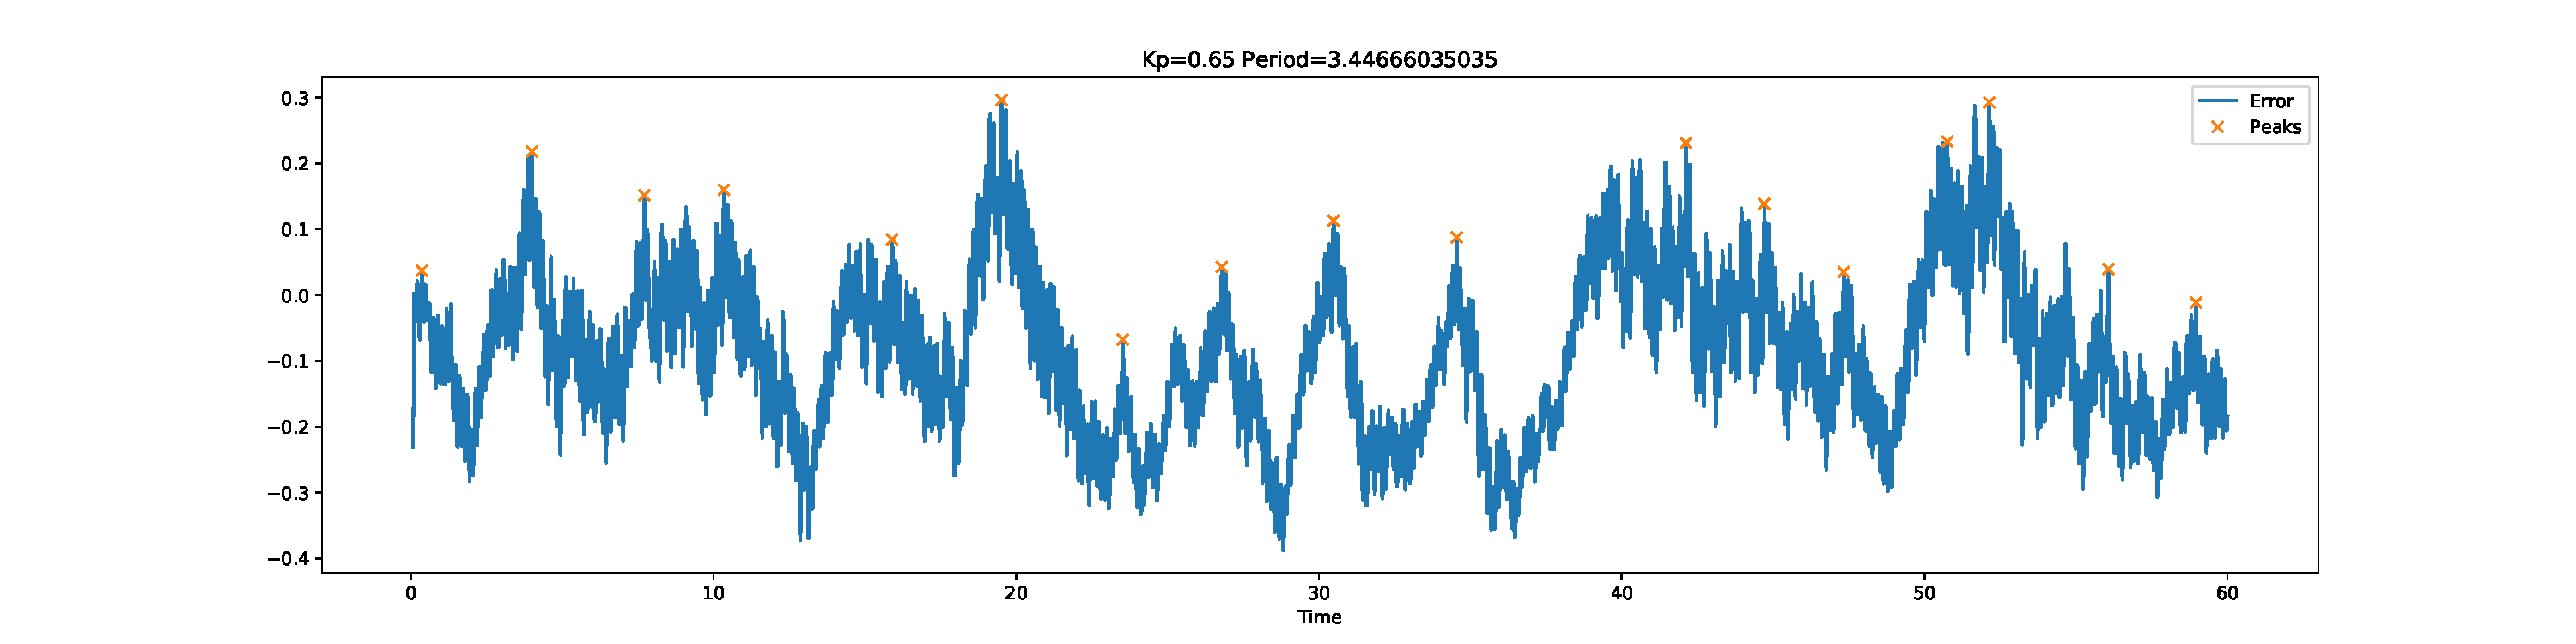
\includegraphics[trim={5cm 0 5cm 0},clip,width=\textwidth]{PIDnoise.pdf} 
\end{figure}

I thought the above graph showed a lot of noise so I added a 1-Dimensional Gaussian filter to help estimate actual error peaks. The filter is also a function of the SciPy library.

\begin{figure}[ht!] % [h] forces the figure to be output where it is defined in the code (it suppresses floating)
	\centering
	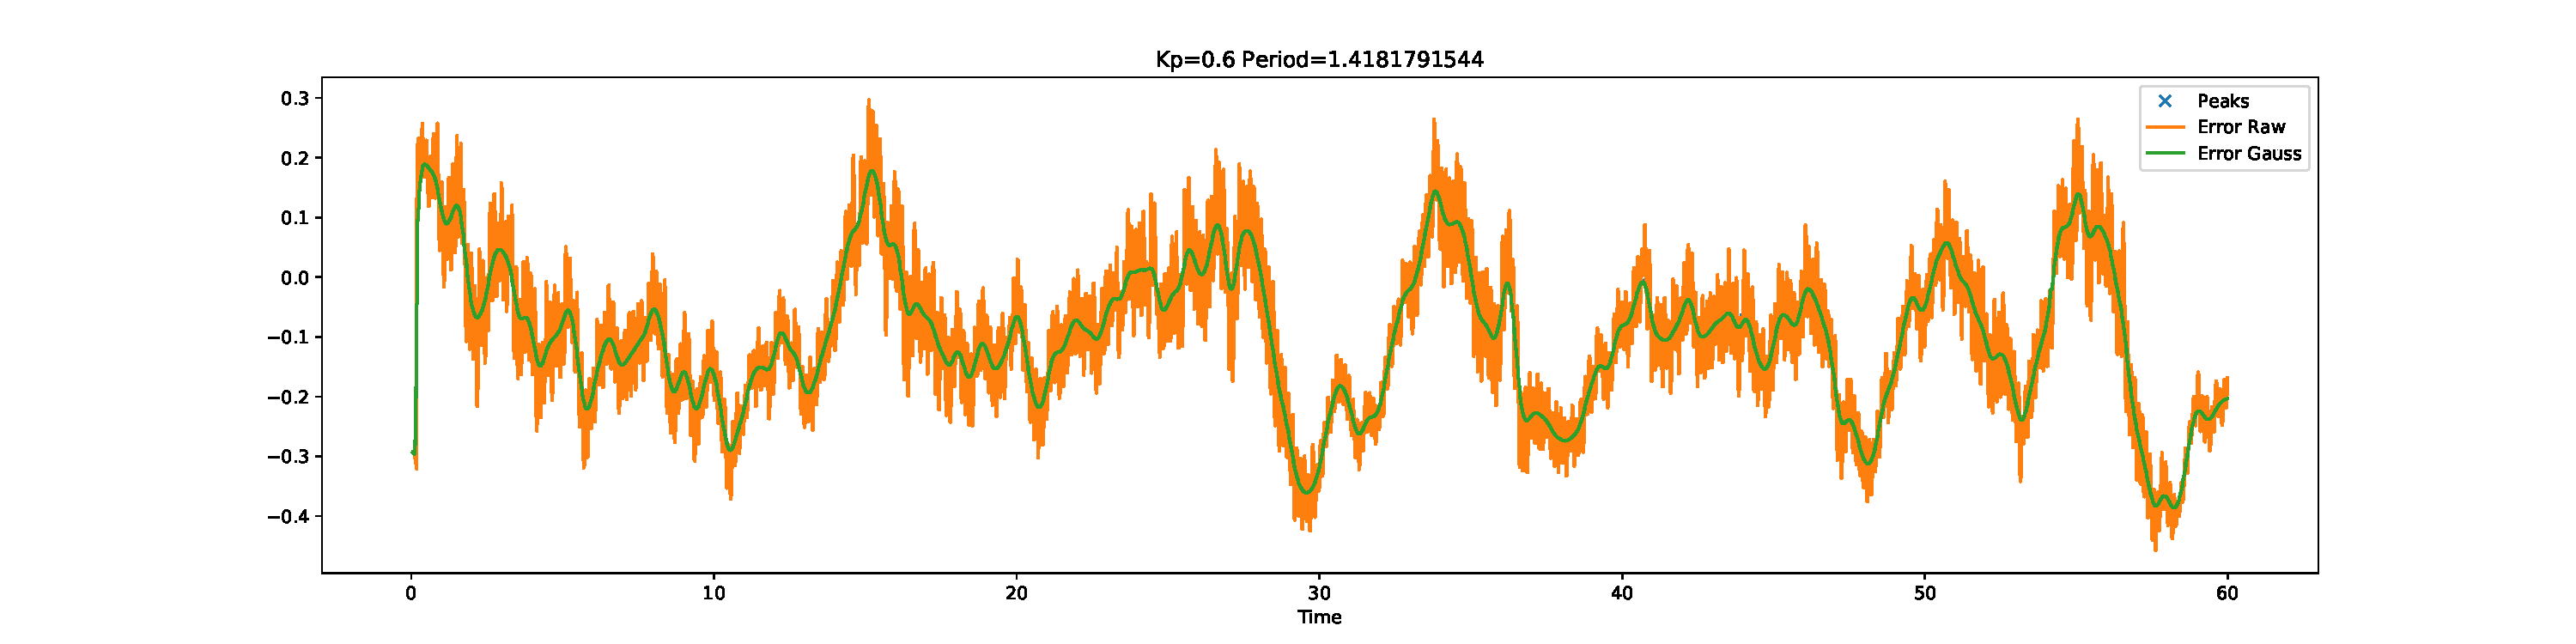
\includegraphics[trim={5cm 0 5cm 0},clip,width=\textwidth]{PIDnoiseGauss.pdf} 
\end{figure}

But it turns out it wasn't noise, but a consequence of using gain values far too high.

\clearpage

\begin{figure}[ht!] % [h] forces the figure to be output where it is defined in the code (it suppresses floating)
	\centering
	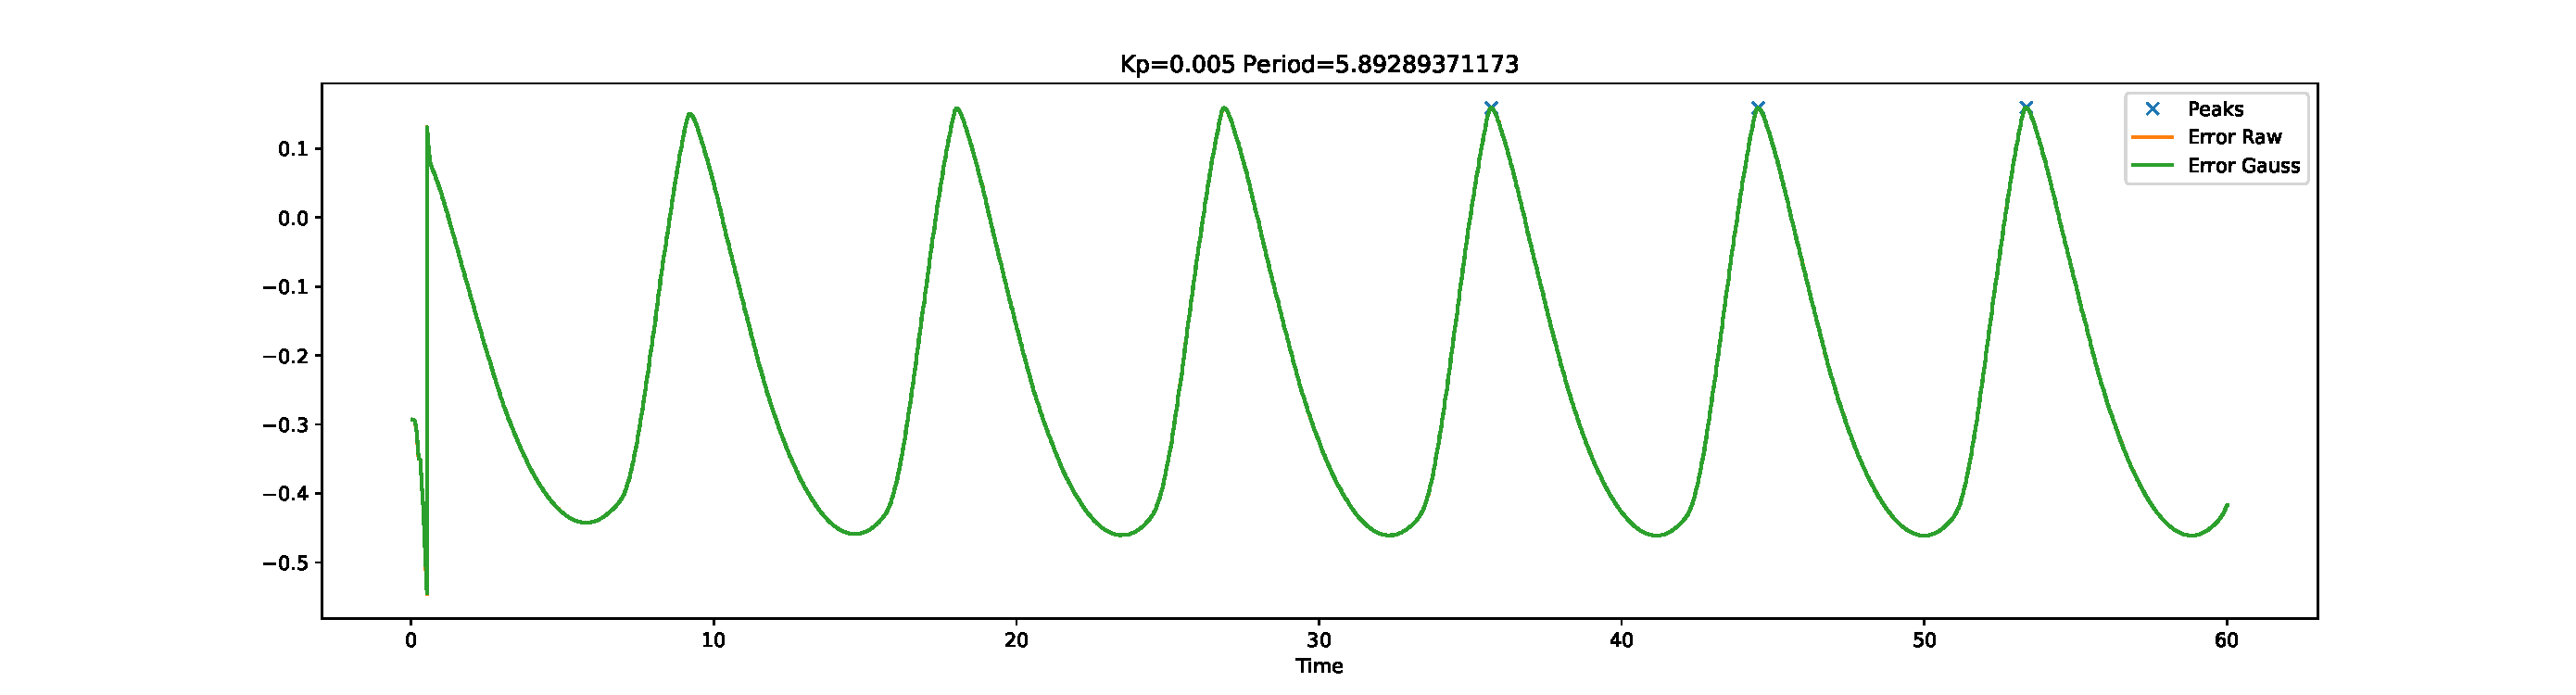
\includegraphics[trim={5cm 0 5cm 0},clip,width=\textwidth]{PIDstalling.pdf} 
\end{figure}

The graph above shows a gain with a steady oscillation, but it is involves the airplane repeatedly stalling.

\begin{figure}[ht!] % [h] forces the figure to be output where it is defined in the code (it suppresses floating)
	\centering
	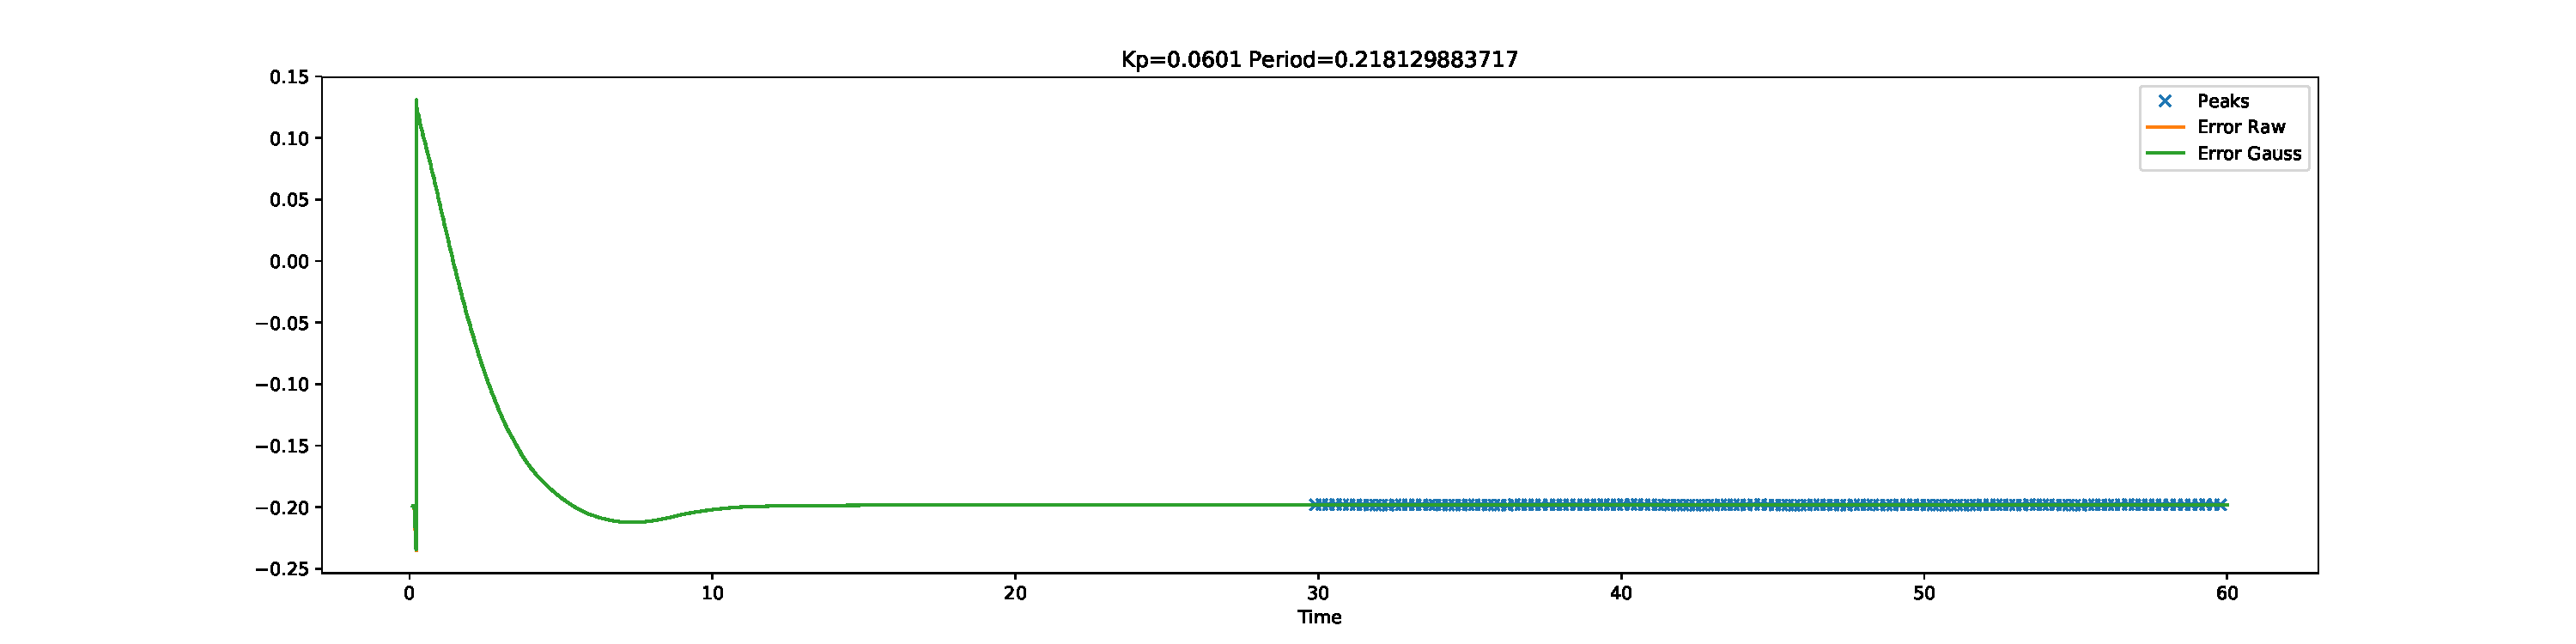
\includegraphics[trim={5cm 0 5cm 0},clip,width=\textwidth]{PIDultimate.pdf} 
\end{figure}

I added a criteria to be minimizing the average distance between the error peaks and troughs and this is the Ultimate gain my final system came up with. The peaks only show on the graph half way through the trial because I set it to analyse after 30 seconds into the trials, allowing it to stabilize before calculating any period.\\

Plugging the ultimate gain into the Ziegler-Nichols formula:
\\
$K_p = 0.7K_u$
\\
$K_i = 1.2K_u/T_u$
\\
$K_d = 0.075K_uT_u$

\begin{figure}[ht!] % [h] forces the figure to be output where it is defined in the code (it suppresses floating)
	\centering
	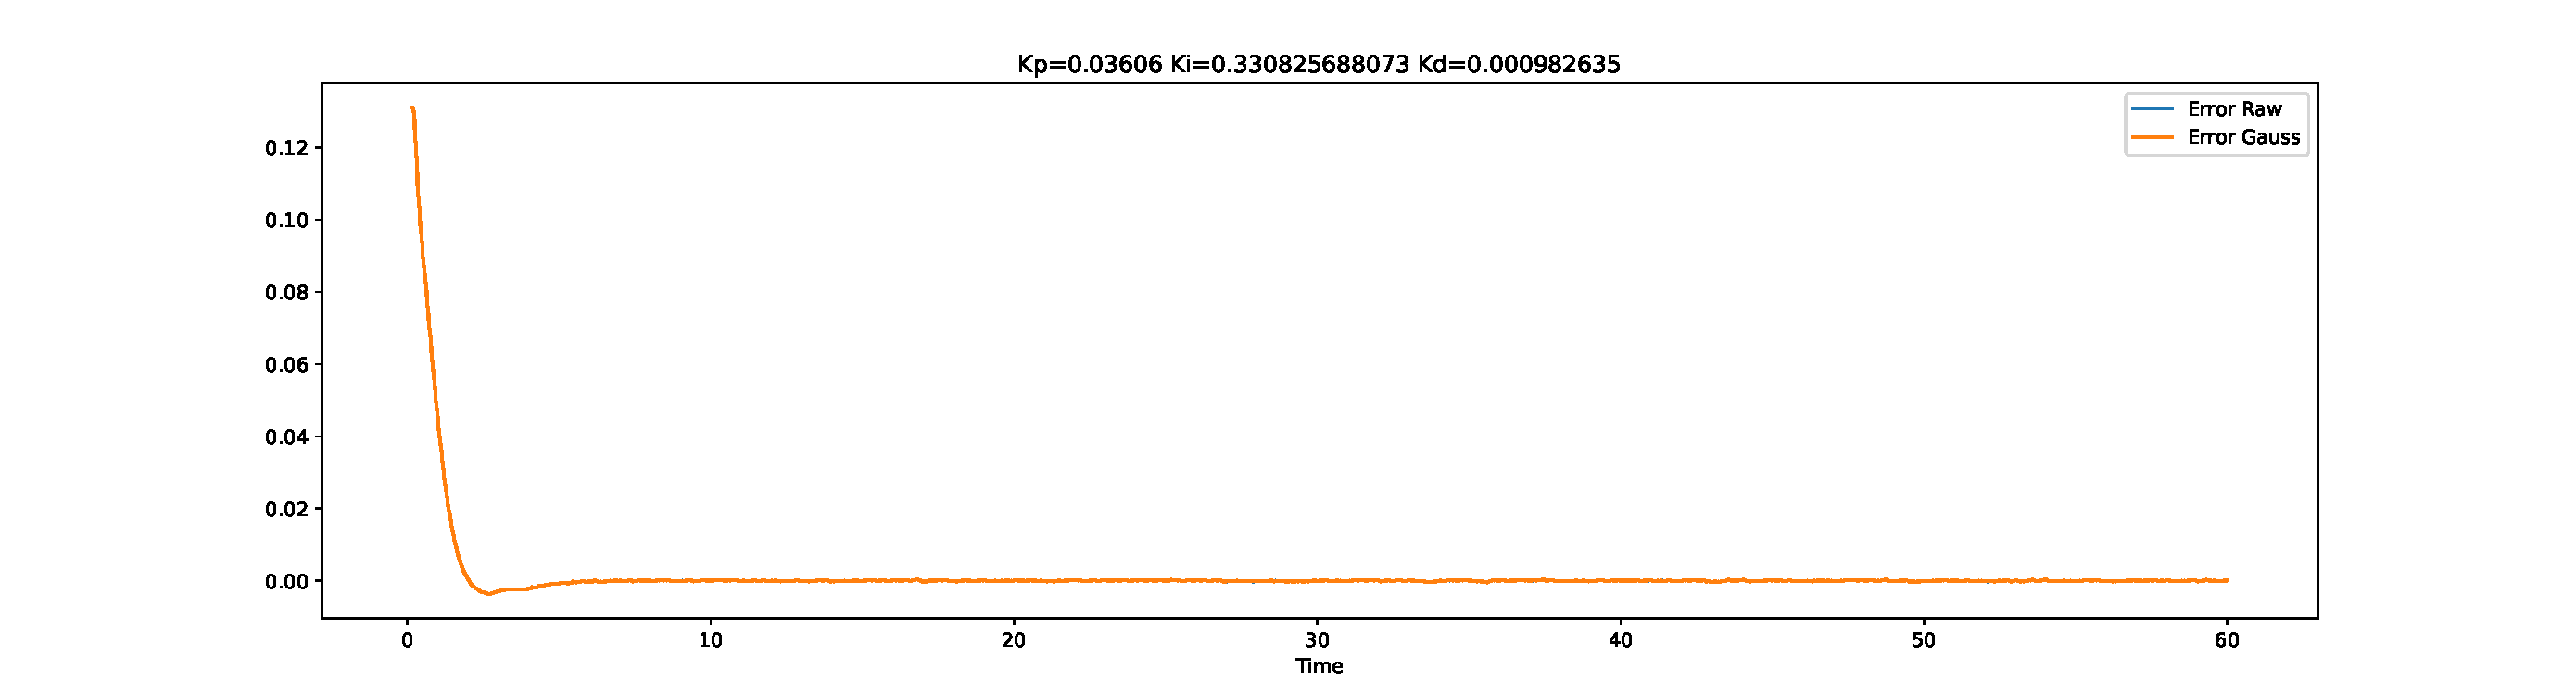
\includegraphics[trim={5cm 0 5cm 0},clip,width=\textwidth]{PIDfinal.pdf} 
\end{figure}

The controller gives minimal overshoot and stabilizes with minimal steady state error. I am very satisfied with this result.
\clearpage

\section{Things to do}
When trying to tune the system I was initially using the rosflight simulated IMU. It has a built in Kalman filter. The filter should get rid of any extraneous errors from the accelerometer and gyroscopic sensors, but even so the attitude would drift about 1 degree every 3 minutes. For a band-aid fix I changed from using the IMU to getting the exact attitude and velocity information from the Gazebo simulation's model. The IMU method will work but I will need to supplement the IMU data with a separate truth reference. I'll try using the simulated magnetometer sensor.\\

After tuning the aileron and rudder PIDs, next term will be focused on integrating the altitude and attitude controllers with the eyebrow detection convolution network. My current plan is to use a quaternion rotation $p'=qpq^{-1}$ to control pitch up/down and bank left/right. I will have the altitude controller do the "neutral" state. \\

I mostly work with embedded C. Therefore I'm still learning a lot about python. Something irritating I've found is that python has no static variables. I got around that by making too many variables global. In the future I will make functions that requires a static variable to be part of a class instead.

\subsection{code}

All files related to this project can be found at:

\url{https://github.com/Trenton-Ruf/Intelligent_Robotics}

\lstinputlisting[
	caption=attitude\_control\_gazebo.py, % Caption above the listing
	%label=lst:test, % Label for referencing this listing
	language=Python, % Use Perl functions/syntax highlighting
	frame=single, % Frame around the code listing
	breaklines=true,
	postbreak=\mbox{\textcolor{red}{$\hookrightarrow$}\space},	
	showstringspaces=false, % Don't put marks in string spaces
	numbers=left, % Line numbers on left
	numberstyle=\tiny, % Line numbers styling
	basicstyle=\footnotesize
	]{../../../catkin_ws/src/rosflight_control/src/attitude_control_gazebo.py}
\clearpage
\medskip

\bibliography{resources.bib}{}
\bibliographystyle{IEEEtran}

\end{document}
